\section{Casting Structured Prediction into Software}\label{sec:api}

Unfortunately only few implementations for learning structured prediction are
publicly available---many applications are based on the non-free implementation
of~\citet{joachims2009cutting}.
In this section, we introduce our implementation, \pystruct, which aims at
providing a high-quality code with an easy-to-use interface, in the high-level
Python language. This allows practitioners to efficiently test a range of
models, as well as allowing researchers to compare to baseline methods much
more easily than this is possible with current implementations. \pystruct is
BSD-licensed, allowing modification and redistribution of the code, as well as
use in commercial applications.  By embracing paradigms established in the
scientific Python community and reusing the interface of the widely-used {\sc
scikit-learn} library~\citep{pedregosa2011scikit}, \pystruct can be used in
existing projects, replacing standard classifiers. The online documentation and
examples help new users understand the somewhat abstract ideas behind
structured prediction.
We base the experiments in the rest of this work on the algorithms
implemented in \pystruct. In the following, we briefly discuss implementation
and features of the \pystruct library.

\subsection{Library Structure and Content}
Using the formulation of structured prediction introduced in
\Secref{basics_structured_prediction}, learning can be broken down into three
sub-problems:
\begin{enumerate*}
    \item Encoding the structure of the problem in a joint feature function $\Phi$.
    \item Solving the loss-augmented prediction problem in Equation~\eqref{loss_augmentation}.
    \item Optimizing the objective in \Eqref{learning_equation} with respect to $\theta$.
\end{enumerate*}
The first two problems are usually tightly coupled, as the maximization in
Equation~\ref{eq:main_equation} is usually only feasible by exploiting the
structure of $\Phi$, as described in \Secref{factor_graphs}. The last problem,
finding $\theta$, on the other hand, is usually treated as independent.
\pystruct takes an object-oriented approach to decouple the task-dependent
implementation of 2. and 3. from the general algorithms used to solve 1.

Estimating $\theta$ is done in \texttt{learner} classes, which currently
support cutting plane algorithms for structural support vector
machines~(SSVMs), the SZLJSP algorithm for SSVMs,
subgradient methods for SSVMs, the structured perceptron and latent variable
SSVMs. See \Secref{learning_algorithms} for a detailed description of the
algorithms. The cutting plane implementation uses the {\sc cvxopt} package
\citep{dahl2006cvxopt} for quadratic optimization.

Encoding the structure of the problem is done using \texttt{model} classes, which
compute $\Phi$ and encode the structure of the problem.
\pystruct implements models for many common cases, such as multi-class and
multi-label classification, conditional random fields with constant or
data-dependent pairwise potentials, and several latent variable models.

The maximization for finding $y$ in Equation~\ref{eq:main_equation} is carried out
using highly optimized implementations from external libraries. \pystruct
includes support for using {\sc OpenGM}~\citep{kappes2013comparative}, {\sc
LibDAI}~\citep{Mooij_libDAI_10}, QPBO fusion moves~\citep{rother2007optimizing},
and {\sc AD$^3$}~\citep{martins2011augmented}. It also includes an interface to
a general purpose linear programming solver from \textsc{cvxopt}~\cite{dahl2006cvxopt}.

Table~\ref{table:comparision_algorithms} and
Table~\ref{table:comparision_models} list learning algorithms and models that
are implemented in \pystruct and compares them to other publicly available
structured prediction libraries.

%TODO what about language / license?
\begin{table}[t]
\centering
\begin{tabularx}{\linewidth}{@{\extracolsep{\fill}}lccccccc}
\toprule
Package       & 1-SP & $n$-SP & SSGD & SZLJSP & L-SSVM & Perceptron & ML\\
\cmidrule(r){1-1} \cmidrule(r){2-8}
\pystruct     & \x   & \x     & \x   & \x   & \x          & \x         & \o\\
\svmstruct    & \x   & \x     & \o   & \o   & \x          & \o         & \o\\
\sc{Dlib}     & \x   & \o     & \o   & \o   & \o          & \x         & \o\\
\sc{CRFsuite} & \o   & \o     & \o   & \o   & \o          & \x         & \x\\

\bottomrule
\end{tabularx}
    \caption{\label{table:comparision_algorithms}Comparison of learning
        algorithms implemented in popular structured prediction software
        packages. 1-CP stands for 1-slack Cutting Plane, $n$-CP for $n$-slack
        Cutting plane, SSGD for stochastic subgradient decent learning of
        SSVMs, SZLJSP is as described in \secref{dual_coordinate_descent},
        L-SVM stands for latent variable SSVMs, and ML for
        maximum likelihood learning.}
\end{table}

\begin{table}[t]
\centering
\begin{tabularx}{\linewidth}{@{\extracolsep{\fill}}lcccccc}
\toprule
Package        &Multi-Class &  Multi-Label & Chain & Graph & LSVM  &LDCRF \\
\cmidrule(r){1-1} \cmidrule(r){2-7}
\pystruct      & \x         & \x           & \x    & \x    & \x    & \x    \\
\svmstruct     & \x         & \x           & \o    & \o    & \o    & \o    \\
\sc{Dlib}      & \x         & \o           & \x    & \x    & \o    & \o    \\
\sc{CRFsuite}  & \o         & \o           & \x    & \o    & \o    & \o    \\

\bottomrule
\end{tabularx}
    \caption{\label{table:comparision_models}Comparison of models implemented
    in popular structured prediction software packages. LSVM stands for the latent multi-class SVM, LDCRF for
    latent dynamic conditional random fields.}
\end{table}

\subsection{Project Goals}\label{sec:goals}

\paragraph{Completeness}
    \pystruct aims at providing complete predictors that can be used directly in
    applications. It contains model formulation for many typical scenarios.
    This is in contrast to \svmstruct that provides no models at all, requiring the
    user to develop significant amounts of code, even for simple tasks.

\paragraph{Modularity}
    \pystruct separates the algorithms for parameter estimation and
     inference from the task-dependent formulation of $\Phi$. This allows
     practitioners, for example in computer vision or natural language
     processing, to improve their model without changing any optimization
     code. On the other hand, researchers working on better inference or
     parameter learning can easily benchmark their improvements on a wide
     array of applications.

\paragraph{Efficiency}
     While \pystruct focuses on usability, providing efficient and competitive
     implementations is important to allow fast prototyping and scaling to
     large datasets. \pystruct achieves the same runtime performance
     as the popular \svmstruct model for cutting plane algorithms, and
     provides implementations of the BCFW and Subgradient methods that scale to
     large datasets.

\paragraph{Documentation and Examples}
     \pystruct provides full documentation of all classes and functions.  It
     also provides examples for many important applications, such as
     sequence tagging, multi-label classification and image segmentation.
     Furthermore, standard benchmarks are included as examples, which allows
     easy comparison with the literature.

\paragraph{Testing}
     \pystruct contains a testing-suite with 80\% line-coverage. It also
     employs continuous integration to ensure stability and a seamless user
     experience.

\paragraph{Integration}
     To improve usability, \pystruct is interoperable with other numeric and
     scientific Python projects, such as {\sc
     scikit-learn}~\citep{pedregosa2011scikit},
     {\sc mahotas}~\citep{coelho:mahotas}, {\sc gensim}~\citep{rehurek_lrec},
     and {\sc scikit-image}.  This allows users to build powerful applications
     with little effort. In particular, most of the model-selection methods of
     {\sc scikit-learn} can be used directly with \pystruct.


\subsection{Usage Example: Semantic Image Segmentation}\label{sec:examples}
%TODO Multi-label, chain?

%\subsection{Multi-class classification}
%Multi-class classification is a very simple case of structured prediction, that serves
%well to exemplify the usage. We load the iris dataset and compare the usage of \pystruct
%with a call to LibLinears Crammer-Singer SVM using scikit-learn.
%\lstinputlisting[language=Python, frame=single, basicstyle=\scriptsize,
    %numbers=left, commentstyle=\color{blue}\normalfont,
%columns=flexible, firstline=11]{multi_class_example.py}
%\subsection{OCR sequence classification}
%Chain structured CRFs are commonly used in natural language processif, for
%example for part-of-speech tagging or named entity recognition.  Here we
%demonstrate the use of a chain CRF on the OCR dataset from. The ChainCRF provides
%a very simnple interface for this problem. Each example is presented as an
%array of input features of shape % (length_of_sequence, number_of_features).
%% listing, training time, accuracy, comparision with kraehenbuehl
%TODO snakes

We demonstrate the use of \pystruct on the task of semantic image segmentation,
the main focus of this work. The example shows how to learn an $n$-slack support
vector machine on a superpixel-based CRF on the popular Pascal dataset. We use
unary potentials generated using TextonBoost
from \citet{krahenbuhl2012efficient}. The superpixels are generated using SLIC~\citep{achanta2012slic}.%
\footnote{The preprocessed data can be downloaded at \url{http://www.ais.uni-bonn.de/download/datasets.html}.}
Each sample (corresponding on one entry of the list \texttt{X}) is represented as a
tuple consisting of input features and a graph representation.
\begin{listing}[t]
\begin{pythoncode}
model = crfs.EdgeFeatureGraphCRF(
            class_weight=inverse_frequency,
            symmetric_edge_features=[0, 1],
            antisymmetric_edge_features=[2],
            inference_method='qpbo')

ssvm = learners.NSlackSSVM(model, C=0.01, n_jobs=-1)
ssvm.fit(X, Y)
\end{pythoncode}
\caption{Example of defining and learning a CRF model.\label{lst:stuff}}
\end{listing}

The source code is shown in Listing 1.
Lines 1-3 declare a model using parametric edge potentials for arbitrary graphs.
Here \texttt{class\_weight} re-weights the hamming loss according to inverse class
frequencies. The parametric pairwise interactions have three features: a
constant feature, color similarity, and relative vertical position. The first two
are declared to be symmetric with respect to the direction of an edge, the last
is antisymmetric. The inference method used is QPBO-fusion moves.  Line 5
creates a \texttt{learner} object that will learn the parameters for the given
model using the $n$-slack cutting plane method, and line 6 performs the actual
learning.  Using this simple setup, we achieve an accuracy of 30.3 on the
validation set following the protocol of \citet{krahenbuhl2012efficient}, who
report 30.2 using a more complex approach. Training the structured model takes
approximately 30 minutes using a single i7 core.

\subsection{Experiments}\label{sec:benchmarks}
While \pystruct focuses on usability and covers a wide range of applications, it is also
important that the implemented learning algorithms run in acceptable time.
In this section, we compare our implementation of the $1$-slack cutting plane
algorithm with the implementation in \svmstruct.
We compare performance of the Crammer-Singer multi-class SVM with respect to
learning time and accuracy on the MNIST dataset of handwritten digits.
While multi-class classification is not very interesting from a structured
prediction point of view, this problem is well-suited to benchmark the cutting
plane solvers, as loss-augmented prediction is trivial.

Results are shown in \Figref{timings}. We report learning times and accuracy for
varying regularization parameter $C$. The MNIST dataset has 60\,000 training
examples, 784 features and 10 classes.%
\footnote{Details about the experiment and code for the experiments can be found on the project website.}
The figure indicates that \pystruct has competitive performance, while using
a high-level interface in a dynamic programming language.

\begin{figure}
\centering
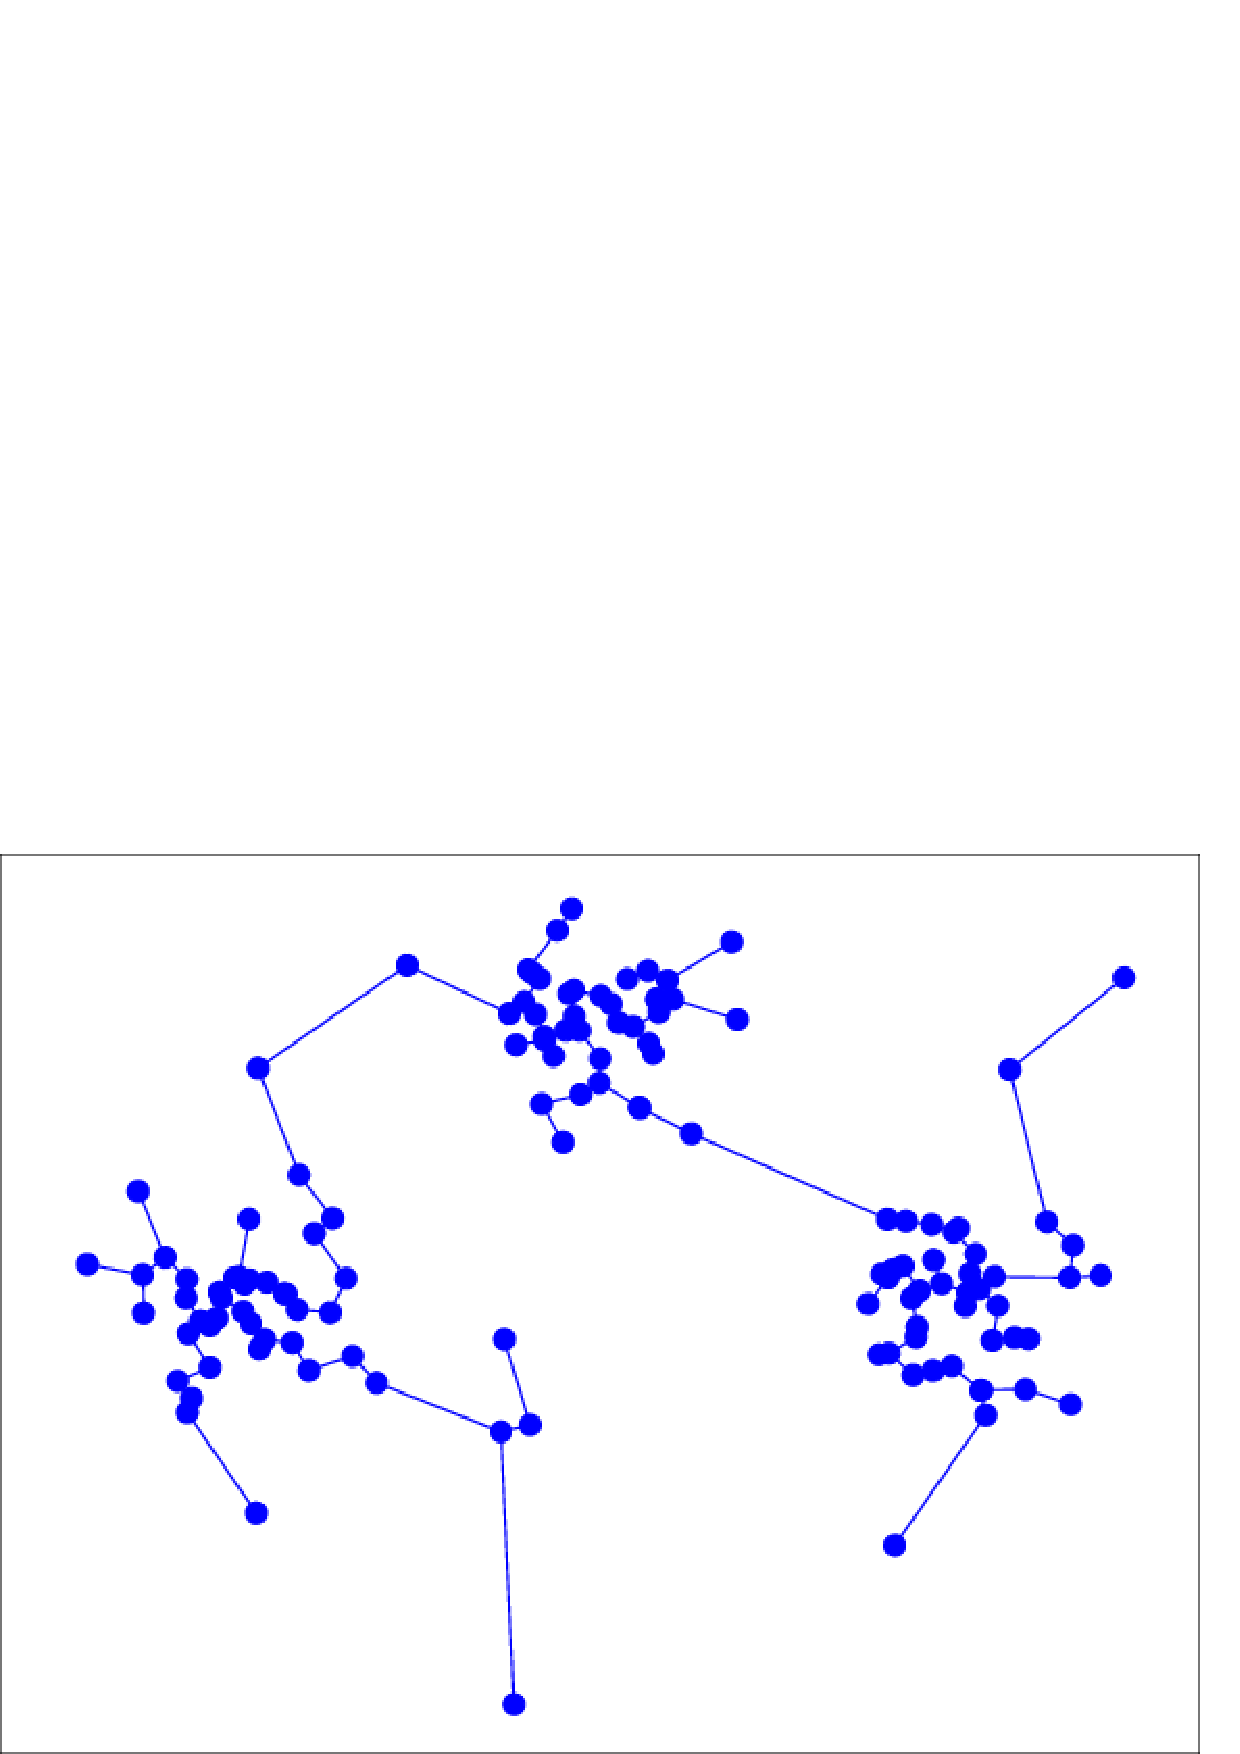
\includegraphics[width=.49\textwidth]{times_MNIST}
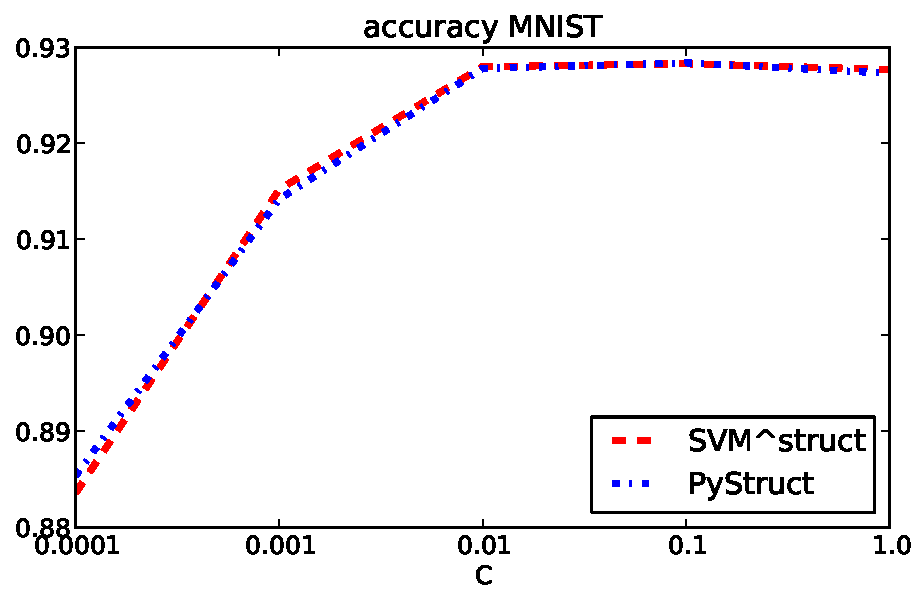
\includegraphics[width=.49\textwidth]{accs_MNIST}
\caption{Runtime comparison of \pystruct and \svmstruct for multi-class
    classification.
}
\label{fig:timings}
\end{figure}

%\section{Comparing Learning Algorithms}
%TODO experiments!!

\section{Summary}
In this chapter, we introduced basic concepts of structured prediction. In particular, we discussed
Structured Support Vector Machines, a max-margin approach for training linear predictors for
structured data. %TODO comparison of algorithms?
We gave a description of several popular learning algorithms, together with their theoretical
runtime bounds and practical considerations.
%TODO summarize structured prediction
We also introduced \pystruct, our modular structured learning and prediction library in Python.
\pystruct is geared towards ease of use, while providing efficient implementations and is be the
basis of our further experiments.
\pystruct integrates itself into the scientific Python ecosystem, making it easy to use with
existing libraries and applications.
Currently, \pystruct focuses on max-margin and perceptron-based approaches.
In the future, we plan to integrate other paradigms, such as sampling-based
learning~\citep{wick2011samplerank}, surrogate objectives (for example
pseudo-likelihood), and approaches that allow for a better integration of
inference and learning~\citep{meshi2010learning}.
